
\documentclass{bredelebeamer}

%%%%%%%%%%%%%%%%%%%%%%%%%%%%%%%%%%%%%%%%%%%%%%%%

\title[Attaques sur connexions HTTPS]{Attaques man-in-the-middle de HTTPS}
\subtitle{SSLStrip, HTTPS-Interception...}
\author[S. Duret - A. Risi - B. Guevel]{Simon Duret \\ Amélie Risi \\ Brendan Guevel}
\institute[]{
  
\includegraphics[scale=0.2]{../medias/universite-bordeaux.pdf}
}

\date{14 mai 2018}

%%%%%%%%%%%%%%%%%%%%%%%%%%%%%%%%%%%%%%%%%%%%%%%%%%%%%%%%%%%%%%%%%%%%%


\begin{document}

%%%%%%%%%%%%%%%%%%%%%%%%%%%
% Titre                   %
%%%%%%%%%%%%%%%%%%%%%%%%%%%
\begin{frame}
  \titlepage
\end{frame}


%%%%%%%%%%%%%%%%%%%%%%%%%%%
% Introduction            %
%%%%%%%%%%%%%%%%%%%%%%%%%%%
\begin{frame}{Introduction}

  {\Large \centerline{HTTP est \emph{le} protocole central du net}}
  \hspace{40cm}

  \begin{columns}
    \begin{column}{0.5\textwidth}
      \begin{itemize}
        % Dire à l'oral que client = navigateur généralement, et serveur = site web
      \item{Assure la transmission des données}
      \item{Architecture client/serveur}
      \end{itemize}
      \begin{alertblock}{Problème}
        \begin{itemize}
        % Donner des exemples à l'oral : interception du wifi, ou physiquement au niveau du cable ethernet, ...
        \item{Tout le trafic est en clair}
        \end{itemize}
      \end{alertblock}

      \begin{exampleblock}{Solution}
        \begin{itemize}
        \item{HTTPS : extension de HTTP}
          % (mot de passe, numéro de carte bancaire, ...)
        \item{Confidentialité et authentification}
        \end{itemize}
      \end{exampleblock}
    \end{column}
    \begin{column}{0.5\textwidth}
      
\includegraphics[width=\linewidth]{../medias/www.png}
    \end{column}
  \end{columns}

  \hspace{20cm}

  {\Large \centerline{Malgré cette protection, des attaques restent possibles...}}


\end{frame}

%%%%%%%%%%%%%%%%%%%%%%%%%%
%  Plan                  %
%%%%%%%%%%%%%%%%%%%%%%%%%%
\begin{frame}{Plan}
  \tableofcontents
\end{frame}

\section{Fonctionnement de HTTP/HTTPS}

%%%%%%%%%%%%%%%%%%%%%%%%%%%
%  Fonctionnement de HTTP %
%%%%%%%%%%%%%%%%%%%%%%%%%%%

\begin{frame}{Fonctionnement de HTTP}
    Procotole de communication client-serveur \\
    Le client demande une ressource à un serveur via une requête HTTP \\
    % Généralement une page html
    Le serveur envoie au client la ressource demandée en réponse \\
    Un navigateur web permet d'automatiser ce processus \\
    De plus ce dernier permet d'afficher la page avec la mise en forme html/css

\end{frame}

%%%%%%%%%%%%%%%%%%%%%%%%%%%
%  Exemple de HTTP        %
%%%%%%%%%%%%%%%%%%%%%%%%%%%

\begin{frame}{Exemple d'une requête HTTP}
    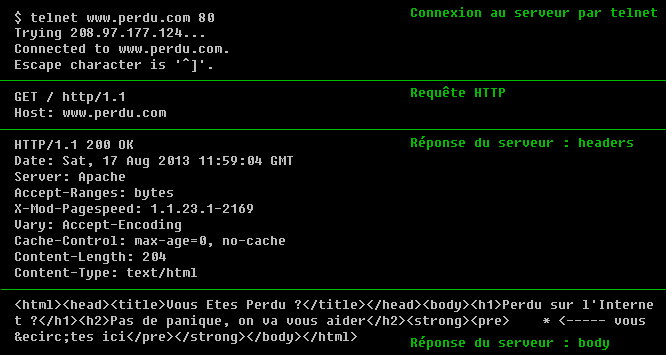
\includegraphics[width=\linewidth]{../medias/perdu.png}
    % Faire une petite démo en live (avec la même requête)
\end{frame}

%%%%%%%%%%%%%%%%%%%%%%%%%%%
%  HTTPS                  %
%%%%%%%%%%%%%%%%%%%%%%%%%%%

\begin{frame}{HTTPS : la version chiffrée de HTTP}
    S pour secure \\
    C'est un deuxième protocole qui est rajouté par dessus HTTP \\
    Historiquement SSL, aujourd'hui remplacé par TLS \\
    Applique un chiffrement sur toute la communication HTTP \\

    Limitation : un attaquant peut toujours voir l'IP/port de destination (nécessaire pour TCP/IP)
\end{frame}


%%%%%%%%%%%%%%%%%%%%%%%%%%%
%  Certificats            %
%%%%%%%%%%%%%%%%%%%%%%%%%%%

\begin{frame}{Gestion des certificats}

\end{frame}

%%%%%%%%%%%%%%%%%%%%%%%%%%%
%  TLS                    %
%%%%%%%%%%%%%%%%%%%%%%%%%%%

\begin{frame}{Le protocole SSL/TLS}
  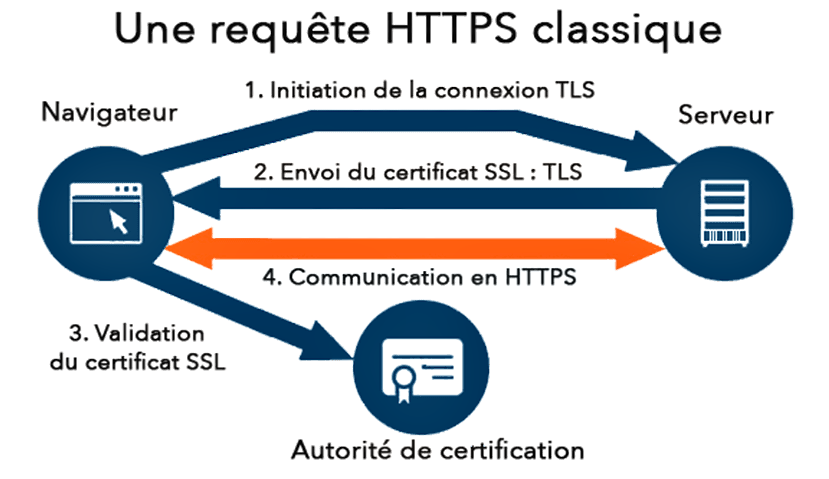
\includegraphics[width=\linewidth]{../medias/protocole-tls.png}
\end{frame}

\section{Etat de l'art}

%%%%%%%%%%%%%%%%%%%%%%%%%%%
%  Attaques HTTPS         %
%%%%%%%%%%%%%%%%%%%%%%%%%%%

\begin{frame}{Attaques sur HTTPS}

  {\Large \centerline{Plusieurs angles d'attaques :}}

  \begin{exampleblock}{Failles d'implémentation}
    \begin{itemize}
    \item Bibliothèques (openssl)
    \item Navigateurs (Internet Explorer)
    \end{itemize}
    \end{exampleblock}

  \begin{exampleblock}{Cryptographie}
    \begin{itemize}
    \item Mode de chiffrement (CBC)
    \item Algorithmes (RC4)
    \end{itemize}
  \end{exampleblock}

  \begin{exampleblock}{Protocole}
    \begin{itemize}
      \item{Downgrade attack (POODLE)}
    \end{itemize}
  \end{exampleblock}

\end{frame}

\begin{frame}{Historique des attaques sur SSL/TLS}
    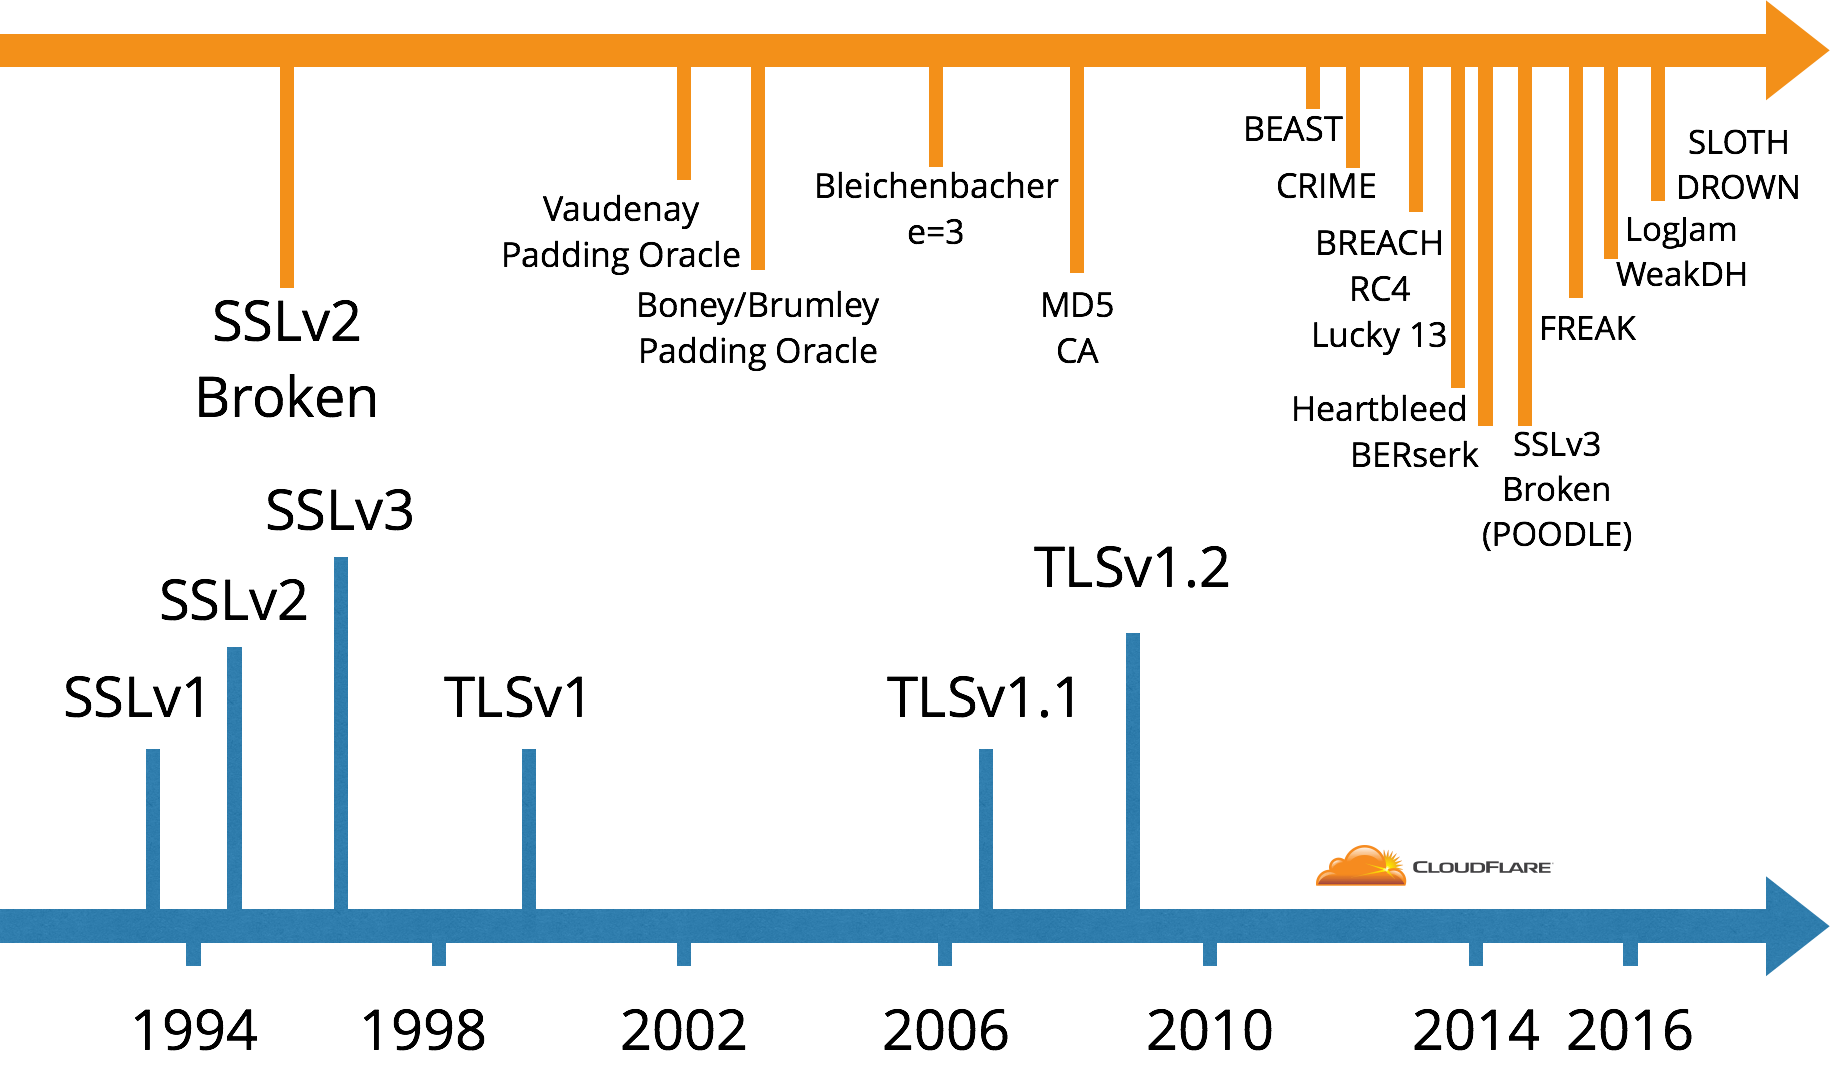
\includegraphics[width=\linewidth]{../medias/history-tls-attacks.png}
\end{frame}

\section{Environnement}

\begin{frame}{Environnement}
    \begin{block}{Qemunet}
		Outil pour créer un réseau virtuel
    \end{block}
\end{frame}

\begin{frame}{Topologie}
    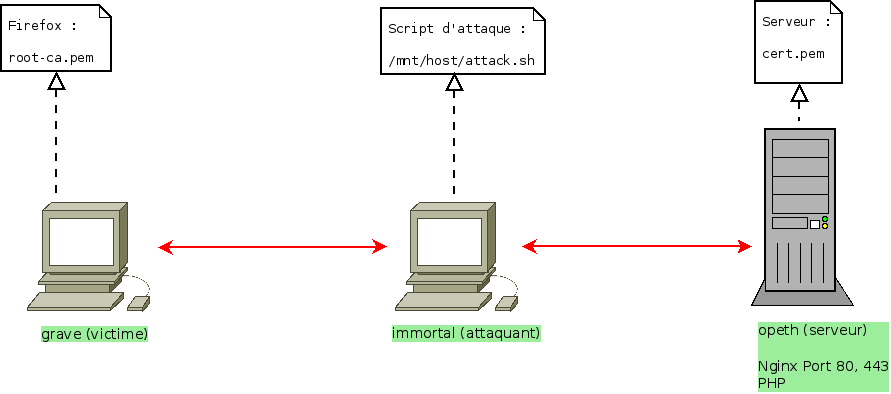
\includegraphics[width=\linewidth]{../medias/topology.png}
\end{frame}

\section{SSLStrip}

\begin{frame}{Fonctionnement d'un lien dans une page html}

\end{frame}

\begin{frame}{Attaque SSLStrip}
    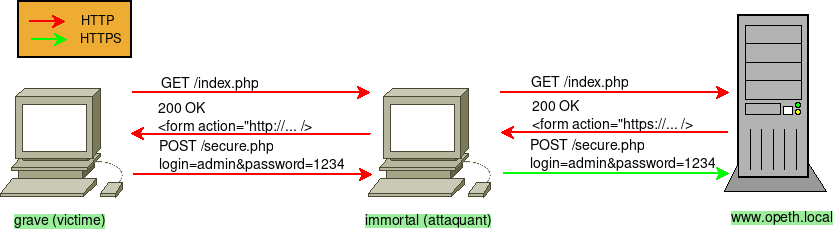
\includegraphics[width=\linewidth]{../medias/sslstrip/attack.png}
\end{frame}

\section{SSLStrip+}

\begin{frame}{Fonctionnement de DNS}
\end{frame}

\begin{frame}{Attaque SSLStrip+}
    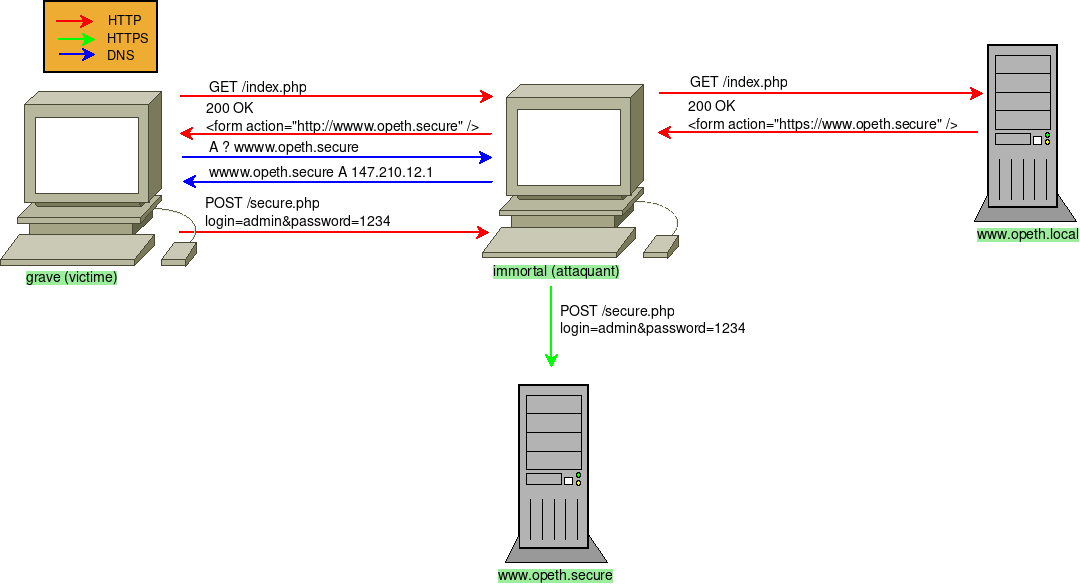
\includegraphics[width=\linewidth]{../medias/sslstrip2/attack.png}
\end{frame}

\section{SSLStrip NTP}

\begin{frame}{Fonctionnement de NTP}
\end{frame}

\begin{frame}{Attaque SSLStrip NTP}
    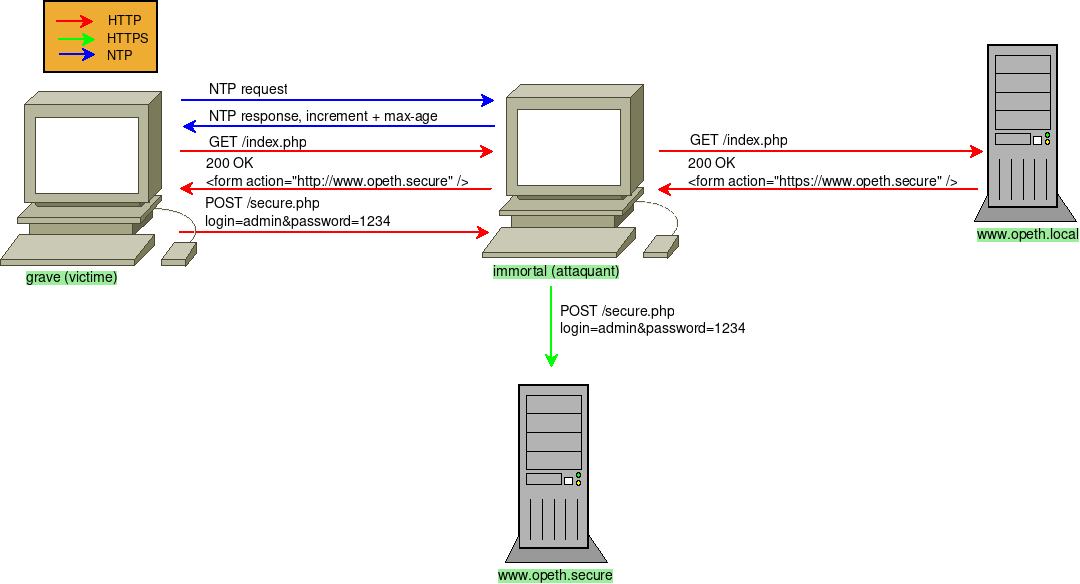
\includegraphics[width=\linewidth]{../medias/sslstrip-ntp/attack.png}
\end{frame}

\section{HTTPS interception}

\begin{frame}{Certificat numérique}
    -> Permet d'authentifier la communication \\
    -> Sur internet, cela sert essentiellement à s'assurer de l'identité du serveur \\
    -> Nécessité d'une authorité de certification (un tiers) \\
\end{frame}

\begin{frame}{Attaque HTTPS interception}
    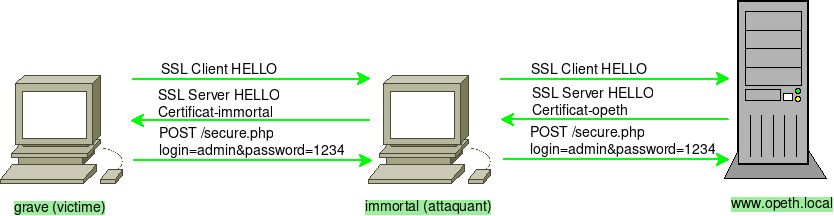
\includegraphics[width=\linewidth]{../medias/https-interception/attack.png}
\end{frame}


\end{document}
